\documentclass[12pt]{article}
\usepackage{latexsym}
\usepackage{fancyhdr}
\usepackage{amssymb,amsmath,amsthm}
\usepackage[pdftex]{graphicx}
\usepackage{pdfpages}
\usepackage[margin=1in]{geometry}


% Create answer counter to keep track of seperate responses
\newcounter{AnswerCounter}
\newcounter{SubAnswerCounter}
\setcounter{AnswerCounter}{1}
\setcounter{SubAnswerCounter}{1}

% Create answer environment which uses counter
\newenvironment{answer}[0]{
  \setcounter{SubAnswerCounter}{1}
  \bigskip
  \textbf{Solution \arabic{AnswerCounter}}
  \\
  \begin{small}
}{
  \end{small}
  \stepcounter{AnswerCounter}
}

\newenvironment{subanswer}[0]{
  (\alph{SubAnswerCounter})
}{
 \bigskip
  \stepcounter{SubAnswerCounter}
}

% Allows easy use of vectors
\newcommand{\vect}[1]{\vec{\boldsymbol{#1}}}

% Setting up the title
\title{Mathematics 131 \\
Topology I}
\author{
        Luis Antonio Perez \\
        HUID: 70871564 \\
        Harvard College \\
        \href{mailto:luisperez@college.harvard.edu}{luisperez@college}
}
\date{\today}

% Custom Header information on each page
\pagestyle{fancy}
\lhead{HUID: 70871564}
\rhead{Perez - \thepage}
\renewcommand{\headrulewidth}{0.1pt}
\renewcommand{\footrulewidth}{0.1pt}

% Title page is page 0
\setcounter{page}{0}

\begin{document}
%\maketitle
\pagebreak
\begin{answer}[Page 171, \#4]
We show that every subspace of a compact metric space is closed.
\begin{proof}
Let $X$ be a metric space. For any $x,y \in X$ where $x \neq y$, we first note that $d(x,y) = \epsilon > 0$. Then $B(x,\epsilon/3)$ and $B(y,\epsilon/3)$ are two open sets containing $x,y$ that separate $x,y$ (this is by the triangle inequality). Therefore every metric space is Hausdorff, and by Theorem 26.3, every compact subspace is closed.
\end{proof}
Next, we show that every subspace of a compact metric space is bounded.
\begin{proof}
For contradiction, suppose we have a compact subspace $Y$ of $X$ (metric) where $Y$ is unbounded. Then for any open covering $\mathcal{U}$, for any point $y \in Y$, there exists an element $U \in \mathcal{U}$ which covers $y$. This element is of the form $B(y,d)$ for some distance $d$. However, note that the open ball is bounded, and therefore this element cannot cover the entire unbounded subspace $Y$. Therefore, $\exists y' \in Y$ such that $y' \notin U$. Since $\mathcal{U}$ is a covering, then $\exists U' \in \mathcal{U}$ such that $y' in U'$. In particular, $B(y',d')$. Note that this collection of open balls covers all of $Y$, but there's no finite sub-covering. This contradict the fact that $Y$ is compact, therefore $Y$ must be bounded.
\end{proof}
Now we find a metric space in which not every closed and bounded subspace space is compact. We can do this relatively easily. Take the space $\mathbb{R}$ with the bounded, discrete metric. (ie, $d(x,x) = 0, d(x,y) = 1$). Then note that $\mathbb{R}$ is bounded, it is closed, but it is not compact.
\end{answer}

\begin{answer}[Page 171, \#7]
Following the hint, we first show that if $Y$ is compact, then the projection $\pi: X \times Y \to X$ is a closed map.
\begin{proof}
Take closed $C \in X \times Y$. We show that $R = \pi(C)$ is also closed by showing $\pi(C)^c$ is open. Take a point $x \in X$ such that $x \notin \pi(C)$. Then note that $x \times Y \subseteq (X \times Y) \setminus C$, which is open. Therefore, by the tube lemma (26.8), there exists some tube $W \times Y$ about $x \times Y$ fully contained in $(x \times Y) \setminus C$ such that $W$ is an open set in $X$ about the point $x$. Therefore, $\pi(C)^c$ is open, so $\pi(C)$ is cloed.
\end{proof}
The above shows that the projection $\pi: X \times Y \to X$ where $Y$ is compact is closed.

Now we prove that if $f: X \to Y$ is continuous and $Y$ is compact Hausdorff, then the graph $G_f = \{ x \times f(x) \mid x \in X\}$ is closed in $X \times Y$.
\begin{proof}
Take a point $(x,y) \in X \times Y$ such that $y \neq f(x)$ and therefore $(x,y) \notin G_f$. Note by the fact that $Y$ is Hausdorff, there exist two open neighborhoods $U$ and $U'$ such that $y \in U$ and $f(x) \in U'$ where $U \cap U' = \emptyset$. Now consider the open set $f(V)$ such that $f(x) \in f(V) \subseteq U'$. Note that by the continuity of $f$, $V$ is open in $X$. Then we have the set $U \times V$, the product of two open sets, must be open in $X \times Y$ and does not intersect the $G_f$, and contains the point $(x,y)$. Therefore $G_f^C$ is open, which implies $G_f$ is closed in $X \times Y$.
\end{proof}

Next, we prove that if the graph $G_f$ is closed in $X \times Y$ where $Y$ is compact Hausdorff, then $f$ is continuous.
\begin{proof}
We show $f$ is continuous by showing that if we take a closed subset $C \subseteq X \times Y$, then $R = f^{-1}(C) \subseteq X$ is also closed. First, suppose $C \cap G_f = \emptyset$. Then $f^{-1}(C)$ is the empty set, which is closed. On the other hand, $f^{-1}(C) = f^{-1}(C \cap G_f)$. Note that $C \cap G_f$ is closed. Furthermore, note that $f^{-1}(C \cap G_f)$ is simply the projection map onto the $x$-coordinate, and with $Y$ compact, we've already shown that $f^{-1}(C \cap G_f)$ is a closed map, therefore $R$ is closed. This implies $f$  is continuous.
\end{proof}
\end{answer}

\begin{answer}[Page 171, \#10]

\begin{subanswer}
Recall the monotone increasing property of $f$, and note that $f(x) \geq f_n(x)$ for all $n$. Take any point $x \in X$. We know that $\forall \epsilon > 0$, there exists $N_x$ large enough such that we have $f(x) - f_{N_x}(x) < \epsilon$. Note that $f(x) - f_{N_x}(x)$ is continuous, as each $f_{N_x}$ and $f$ are continuous, and therefore we have the property that there exists some $\delta > 0$ such that for all $x' \in B(x, \delta_x)$, $f(x') - f_{N_x}(x') < \epsilon$. Furthermore, note that the above holds for all $n > N_x$ because $f_{N_x} < f_{n}(x)$ by the monotonicity of $f_n$.

Now take the collection of such balls, $B(x,\delta_x)$ for all $x \in X$. This collection forms an open covering of $X$. By compactness, there exists a finite sub-covering $B(x_i,\delta_{x_i})$ that covers $X$. Then take $N = \max\{N_{x_i}\}$, and note that $\forall x \in X$, by the covering property, $x \in B(x_i, \delta_{x_i}$ for some $x_i$. Therefore, for all $n \geq N$ $f(x) - f_n(x) <\epsilon$. This proves uniform continuity.
\end{subanswer}

\begin{subanswer}
If we delete the requirement that $X$ be compact, then we can take the sequence of piecewise continuous functions:
\begin{align*}
f_n(x) &=
\begin{cases}
0 &= x \leq n \\
n - x &= x > n
\end{cases}
\end{align*}
Note that the above sequence, by construction, converges to the $0$ function. Furthermore, the sequence is monotone increasing (for $ x > n$, $f_n(x) < 0$ but as $n$ increases, $f_n(x)$ eventually becomes $0$). However, it does not converge uniformly. For any $n$, the point $f_n(n + 1) = 1$.

On the other hand, if we delete the requirement that the function be monotone increasing, we can take the function sequence given by Exercise 9 in Section 21:
\begin{align*}
f_n(x) &= \frac{1}{n^3[x - \frac{1}{n}]^2 + 1}
\end{align*}
where we restrict $f_n: [0,1] \to \mathbb{R}$. Then note that $[0,1]$ is compact. However, as shown in Exercise 9, this sequence does not converge uniformly to to the zero function.
\end{subanswer}
\end{answer}

\begin{answer}[Page 171, \#11]
We follow the hint relatively closely. We use proof by contradiction. Suppose non-connectivity, and let $C,D$ be a separation of $Y = \bigcap_{A \in \mathcal{A}} A$ where $\mathcal{A}$ is ordered by proper inclusions and each $A$ is closed and connected. Note that each $A$ is closed, so $Y$ is closed. Therefore $C,D$ are both closed, and since $X$ is Hausdorff compact, $C,D$ are compact. Now we show that there exist disjoint open sets $U,V$ containing each $C,D$.
\begin{proof}
For each $c \in C$, and each $d \in D$, by Hausdorff, there exists two disjoint open sets $U_c,V_d$ such that $c \in U_c$ and $D \subseteq V_c$. Note that the collection of $U_c$ forms an open covering of $C$. By compactness, there exists a finite sub-cover, $\{ U_{c_i}\}$. Then note that the finite intersection of the corresponding $V_{c_i}$ is open (because it's finite), and $\bigcap V_{c_i} \cap \bigcup U_{c_i} = \emptyset$. Therefore we have found two disjoint open sets $U = \bigcup U_{c_i}$ and $V = \bigcap V_{c_i}$ which cover $C$ and $D$ respectively.
\end{proof}
Next, we proof that the above implies the existence of a point $y \in Y$ such that $y \notin U \cup V \implies y \notin C \cup D$ which contradicts the assumption that $C,D$ form a separation. We do this by showing that the intersection of the sets $A \in \mathcal{A}$ after removal of $U,V$ is non-empty.
\begin{proof}
Consider the set $E = Y - (U \cup V)$, which we will show is non-empty. We can re-write this as:
$$
E = \bigcup_{A \in \mathcal{A}} A - (U \cup V) = \bigcap_{A \in \mathcal{A}} (A - (U \cup V))
$$
Note that $A - (U \cup V) = A \cap (X - (U \cup V))$ which is closed. Furthermore, using the property that each $A \in \mathcal{A}$ is property nested, we have that each $A - (U \cup V)$ is also properly nested. Finally, note that each $A$ is connected, and therefore $A - (U \cup V)$ must be non-empty. If it were empty, then we'd have $U \cup V \supset A$ would be a separation of $A$.

Then by the compactness of $X$, it must be the case that this uncountable intersection is non-empty.
\end{proof}
Taken together, the above shows that our assumption that there exists a separation of $C,D$ leads to a contradiction where not all elements of $Y$ are contained in $C,D$. Therefore, our assumption must be wrong and it must be the case that $Y$ is connected.
\end{answer}

\begin{answer}[Page 177, \# 2]
We let $X$ be a metric space with metric $d$ and we consider the non-empty sub-space $A \subseteq X$.

\begin{subanswer}
We first show that $d(x,A) = 0$ if and only if $x \in A$.
\begin{proof}
Note that $d(x,A) = \inf\{d(x,a) \mid a' \in A\} = 0$ if and only if $\forall \epsilon > 0$, $B(x,\epsilon) \cap A \neq \emptyset$ (otherwise $d(x,A) \geq \epsilon$). However, the above is the case if and only if $x \subseteq \bar{A}$. Therefore $d(x,A) = 0$ iff $x \in \bar{A}$.
\end{proof}
\end{subanswer}

\begin{subanswer}
Now we show that if $A$ is compact, then $d(x,A) = d(x,a)$ for some $a \in A$.
\begin{proof}
The proof is simple. We know $d: X \times X \to \mathbb{R}$ is continuous, therefore $d: X \times A \to \mathbb{R}$ is also continuous. Since it is continuous, it must be continuous on each variable, so for fixed $x \in X$, the function $d_x: A \to \mathbb{R}$ given by $d_x(a) = d(x,a)$ is continuous. Therefore, by compactness of $A$, $d_x$ reaches its minimum for an $a \in A$. This shows that $d(x,a) = d(x,A)$ for some $a \in A$ if $A$ is compact.
\end{proof}
\end{subanswer}

\begin{subanswer}
We show that $\epsilon$-neighborhood of $A$, $U(A,\epsilon)$, is equal to $\bigcup_{a \in A} B(a,\epsilon)$.
\begin{proof}
Take $x \in \bigcup_{a \in A} B(a, \epsilon)$, then $d(x,A) < \epsilon$. Therefore $x \in U(A,\epsilon)$. Similarly, take $x \in U(A,\epsilon)$, then $d(x,A) < \epsilon \implies \exists a \in A$ such that $x \in B(a,\epsilon) \implies x \in \bigcup_{a \in A} B(a,\epsilon)$.
\end{proof}
\end{subanswer}

\begin{subanswer}
We show that if $A$ is compact, then $\exists \epsilon > 0$ such that $U(A,\epsilon) \subseteq U$ where $U$ is an open set containing $A$.
\begin{proof}
We construct a covering of $A$ as follows. For each $a \in A$, consider the ball $B(a,r_a)$ for $r_a > 0$ such that $B(a,2r_a) \subseteq U$ (this is possible because $A \subseteq U$ and $U$ is open). Then note that by compactness, we can take a finite sub-cover of $B(a_i, r_{a_i})$ of $A$. Now we take $\epsilon = \min\{r_{a_i}\} > 0$ and consider $U(A,\epsilon)$. Then note that for any point $p \in U(A,\epsilon)$, $\exists a_i$ such that $B(p,\epsilon) \subseteq B(a_i, r_{a_i} + \epsilon) \subseteq B(a_i, 2r_{a_i}) \subseteq U$. Therefore $p \in U$.
\end{proof}
\end{subanswer}

\begin{subanswer}
If $A$ is not compact, then we don't necessarily have a finite sub-covering, so $\min\{r_i\}$ could equal $0$. For an example of this, we can take the subspace of $\mathbb{R} \times \mathbb{R}$ given by $\{(x,e^{-x}) \mid x \in \mathbb{R}\}$. Note that the open set $(-\infty, \infty) \times (0,\infty)$ contains our subspace. However, because $\lim_{x \to \infty} e^{-x} = 0$, there's no $\epsilon$-neighborhood around the line which is fully contained within the open set.
\end{subanswer}
\end{answer}

\begin{answer}[Page 213, \#4]
Recall that $A$ is a $G_{\delta}$ set in $X$ if $A$ is the intersection of a countable collection of open sets of $X$ (where $X$ is normal). We show that $\exists$ a continuous function $f: X \to [0,1]$ such that $f(x) = 0$ for $x \in A$ and $f(x) > 0$ for $x \notin A$ if and only if $A$ is a closed $G_{\delta}$ set.

We proof that if $A$ is a closed $G_{\delta}$ set, then $\exists$ a continuous function $f: X \to [0,1]$ such that $f(x) = 0$ for $x \in A$ and $f(x) > 0$ for $x \notin A$.
\begin{proof}
Suppose that $A$ is closed, and also the countable intersection of a collection of open sets $\{A_n\}_{n=2}^{\infty}$. Take this countable intersection and add $A_1 = X$ (this does not change it's properties). Then we will define sets $U_p$ such that they fulfill the requirements of the sets used by Urysohn's Lemma as well as to allow us to show that $f^{-1}(0) = A$. First, let $U_1 = A_1$, and for each $n > 1$, define $U_{\frac{1}{n}}$ such that:
$$
A \subset U_{\frac{1}{n+1}} \subset \bar U_{\frac{1}{n+1}} \subset U_{\frac{1}{n}} \cap V_{n+1}
$$
This is possible by the normality of $X$ and by the fact that $A$ is closed. In order to define the remaining $U_p$, we construct the sequence $P_n$ slightly differently. We consider only $p \in \mathbb{Q} \cap (0,1]$. As we did above, starting with $n = 1$, we have $U_1 = A_1$, and then continue to $n = 2$ and define $U_{\frac{1}{2}}$ such that if fulfills the property established previously (it's outside $A$ but inside $V_2 \cap U_1$). Next, we construct all $U_p$ where $\frac{1}{2} < p < 1$.

In general, once we've constructed all $U_p$ for $\frac{1}{n} \leq p \leq 1$, we construct $U_{\frac{1}{n+1}}$ as defined above such that $A \subset U_{\frac{1}{n+1}} \subset \bar U_{\frac{1}{n+1}} \subset U_{\frac{1}{n}} \cap V_{n+1}$ (we have the $U_n$ become subsets of $V_{n+1}$ but still fulfill the properties required by Urysohn Lemma). We then proceed to construct $U_p$ for $\frac{1}{n+1} < p < \frac{1}{n}$ in the same fashion as in Urysohn's Lemma.

In this fashion, we define $U_p$ for all points $p \in \mathbb{Q} \cap (0,1]$.

We then take this collection of $\{ U_p\}$ and use them to define a continuous function $f : X \to [0,1]$ as follows. We define:
\begin{align*}
f(x) &= \inf \{ p \mid x \in U_p \}
\end{align*}
and now we show this is the desired function. First, note that for all $a \in A$, then $a \in U_p$ for all $p > 0$, and therefore $f(a) = 0$ by the denseness of the rationals. We therefore have:
$$
A \subset f^{-1}(0)
$$
Next, note that $f^{-1}(0) \subset \bigcap_{p > 0} U_p$ by definition of $f$. However, note that $\bigcap_{p > 0} U_p \subset \bigcap_{n=1}^{\infty} A_n = A$
\begin{align*}
A \subset f^{-1}(\{0\})
\end{align*}
Taken together
$$
A \subset f^{-1}(0) \subset \bigcap_{p > 0} U_p \subset \bigcap_{n=1}^{\infty} A_n = A \implies A = f^{-1}(0)
$$
We've therefore shown that $f(x) = 0$ if and only if $x \in A$, and therefore $f(x) > 0$ for all $x \notin A$.

Continuity of $f$ follows in the same way as in the proof of The Urysohn Lemma since each of our $U_p$ fulfill all the required properties.
\end{proof}

Next, we proof that if $\exists$ a continuous function $f: X \to [0,1]$ such that $f(x) = 0$ for $x \in A$ and $f(x) > 0$ for $x \notin A$, the $A$ must be a $G_{\delta}$ set (the intersection of a countable collection of open sets).
\begin{proof}
Note that $A = f^{-1}(\{0\})$, so by continuity of $f$, it must be closed. Therefore, we just need to show that $f^{-1}(0)$ can be written as the countable intersection of open sets. To do this, we prove the more general case, showing that for a normal sub-space $A \subset X$ and a continuous function $f: X \to [0,1]$ where $f(x) = 0$ if $x \in A$ and $f(x) > 0$ otherwise:
$$
f^{-1}(r) = \bigcap_{p > r} U_p - \bigcup_{q < r} U_q
$$
where $U_p$ are constructed in the same way as in the proof of Urysohns lemma. Note that the function $f$ above satisfies the properties of the function $g$ used in Urysohns lemman with $B = f^{-1}(1)$.

First, suppose we have $C = f^{-1}(r) \implies f(C) = r$. Then following the proof in the Urysohn Lemma, for each $c \in C$, we have $f(c) = r$ Then note that $c \in \bar{U_r}$, which means $c \in U_p$ for $p > r$, and $b \notin U_q$ for $q < r$. From the above argument, we have that:
$$
C = f^{-1}(r) \subseteq \bigcap_{p > r} U_p - \bigcup_{q < r}U_q
$$
For the other direction, suppose that $b \in U_p$ for all $p > r$. This implies that $f(b) \leq r$. Similarly, if $b \notin U_q$ for all $q < r$, then $f(b) \geq r$. Therefore, $f(b) = r$. We now have the other inclusion, so this proves equality of the two sets.
From the above, we have that:

\begin{align*}
A &= f^{-1}(\{0\}) \\
&= \bigcap_{p > 0} U_p - \bigcup_{q < 0} U_q \tag{definition from above} \\
&= \bigcap_{0 < p \leq 1} U_p \tag{$U_q = \emptyset$ for $q < 0$ and $U_p = X$ for $p > 1$}
\end{align*}
Therefore, $A$ is a closed $G_{\delta}$ set since it is the countable intersection of open $U_p$.
\end{proof}
\end{answer}

\begin{answer}[Page 218, \#3]
Let $X$ be a compact Hausdorff space. We show that $X$ is metrizable if and only if $X$ has a countable basis.
First, the forward direction of the proof. We show that if $X$ is compact and metrizable, then $X$ has a countable basis.
\begin{proof}
Let $d$ be the metric of $X$. Then for each fixed $n$, consider the collection of open balls $\mathcal{A}_n = \{ B_d(x,\frac{1}{n}) \mid x \in X \}$ which forms a covering of $X$. By compactness, there exists a finite sub-cover for each such covering, label it $\mathcal{A}_n'$. Then note that $\mathcal{B} = \bigcup_{n=1}^{\infty} A_n$. We show that $\mathcal{B}$ is a basis for the space $X$ under the induced topology by $d$.
\begin{itemize}
\item By the fact that $\mathcal{B}$ contains sub-covers of $X$, the first property for a basis is trivial.
\item Now, suppose that we have the points $x, x_1, x_2 \in X$ where $x \in B_d(x_1,\frac{1}{n_1}) \cap B_d(x_2, \frac{1}{n_2})$, which is an open set. Therefore, $\exists \epsilon > 0$ such that $B_d(x,\epsilon) \subset B_d(x_1, \frac{1}{n_1}) \cap B(x_2, \frac{1}{n_2})$. Then note that we can choose $N$ large enough such that $\frac{1}{N} < \frac{\epsilon}{2}$. Then note that $\exists U \in \mathcal{T}$ such that $U = B_d(x',\frac{1}{N})$ and $x \in U$ (generated when we considered the $\mathcal{A}_N$ cover of $X$). Then note that $U \subset B(x,\epsilon)$ because $\forall y \in U$:
$$
d(y,x) \leq d(y,x') + d(x',x) < \frac{\epsilon}{2} + \frac{\epsilon}{2} = \epsilon
$$
Therefore,  we have the $\exists$ $B(x',\frac{1}{N} \subset B(x_1,\frac{1}{n_1}) \cap B(x_2,\frac{1}{x_2})$ that contains $x$.
\end{itemize}
With the above, we've show that if $X$ is compact and metrizable, then $X$ has a countable basis (we explicitly construct such a basis).
\end{proof}

Now we show the backwards direction (ie, if $X$ has a countable basis, then it metrizable). We do this by first showing that $X$ is regular (because it is Hausdorff compact), and then by Theorem 34.1, if it has a countable basis, it is metrizable.
\begin{proof}
First, we show that a compact Hausdorff space is regular. Let $x \in X$ and $B \subset X$ closed with $x \notin B$. Then we know $B$ is compact because $X$ is Hausdorff compact. For each point $b \in B$, we consider the disjoint open sets $U_b, V_b$ where $b \in U_b$ and $x \in V_b$ (by Hausdorff property). Then note that $\bigcup_{b \in B} U_b$ forms an cover of $B$, so by compactness, $U = \bigcup_{b_i \in B} U_{b_i}$ is a finite sub-cover of $B$. Then take the corresponding $V \bigcap_{b_i \in B}V_{b_i}$, and note that the set is open. Then $B \subset U$ and $x \in V$ with $U \cap V = \emptyset$. Therefore a compact Hausdorff space is regular.

Now we show that a compact Hausdorff space is normal. Let $X$ be compact Hausdorff. Then take disjoint closed sets $A, B \subset X$. Note that each $A,B$ are compact by Hausdorff compactness of $X$. For each point $a \in A$, there exists disjoint open sets $U_a, V_a$ containing $a$ and $B$ (respectively) by regularity of $X$. The collection $\{U_a\}$ covers $A$, so by compactness of $A$, we can take the set $U = \bigcup_{a_i \in A} U_{a_i}$, open, and the set $V = \bigcap_{a_i \in A} V_{a_i}$, also open. Therefore, this shows the space is normal.

We now conclude using Theorem 34.1 (Urysohn metrization theorem). If $X$ is Hausdorff compact, then it is normal, and if additionally we have a countable basis, then by the Theorem, it is metrizable.
\end{proof}
\end{answer}

\begin{answer}[Problem 1]
Today we will learn more about ``compactness''. First, let's recall a couple of definitions which will help us in understanding compactness.

\textbf{Definition:} A collection $\mathcal{A}$ of subsets of a space $X$ is said to \textbf{cover} $X$, or to be a \textbf{covering} of $X$, if the union of the elements of $\mathcal{A}$ is equal to $X$. It is called an \textbf{open covering} of $X$ if its elements are open subsets of $X$.

The definition is intuitive. You have some space $X$, and then what you do is you take a bunch of other sets, this is the collection, that when you overlap all of them together, they completely cover $X$. You can see Figure \ref{fig:cover} for an image of this.

\textbf{Definition:} A space $X$ is said to be \textbf{compact} if every open covering $\mathcal{A}$ of $X$ contains a finite subcollection that also covers $X$.

This is a relatively strange definition of compact, but it makes sense. Compactness measures how tightly a space is packed, intuitively, and what we have here is a claim that no matter how I cover it, the space $X$ is packed tightly enough that a lot of my open sets are redundant (they cover points already covered by other open sets in the cover). In $\mathbb{R}$, recall that a closed, bounded set is compact.

\begin{figure}[h!]
\centering
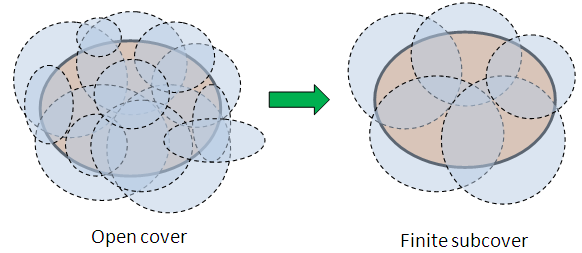
\includegraphics[scale=0.7]{compact_spaces}
\caption{We have a compact space $X$ (colored orange) and we cover it with an infinite number of open sets (colored blue). Next, we extract a finite sub-cover because the space is compact.}
\label{fig:cover}
\end{figure}

However, if you think the above definition is strange, the one we're learning today is even stranger. In order to discuss it, we first need another definition.

In the same way that we defined a ``cover'' above, (as a collection of sets that fulfills a particular property), we'll say that a collection $\mathcal{C}$ has the \textbf{finite intersection} property if for every finite sub-collection of $\mathcal{C}$, the intersection of all of the sets in the sub-collection is non-empty.

How can we think about this? Well, pictures are always worth more than words, so let's try to have a visual for this. We start with a collection of sets $\mathcal{C}$. Imagine these as just a bunch of blobs in some space, for example. Then this collection has the finite intersection property if I can take any finite number of blobs, and they always overlap. Now, this doesn't mean that all of the blobs must overlap! Can you think of a way to imagine the case where not all of the blobs overlap, but any finite number of them do?

Let's see if you get the definition by trying a couple of questions.

\begin{enumerate}
\item Can the empty set be a member of a collection that has the finite intersection property? A: No. Any sub-collection which contains the empty-set will trivially have an empty intersection.
\item Suppose the intersection of all the sets in the collection is non-empty. Does this collection satisfy the finite intersection property?
\item What about the collection $\mathcal{C} = \{ (0,\frac{1}{n}) \mid n > 0 \}$?
A: This satisfies the finite intersection property. The intersection of all the sets is empty, but for any finite collection, the intersection is $(0,\frac{1}{N})$ where $N = \max\{ n_i \}$ for the $n_i$ selected subsets.
\item Can you generalize the above? Let's say your collection is nested? A: A nested collection satisfies the finite intersection property.
\item Take $X = (0,1)$. Define the collection $\mathcal{C}$ such that $\mathcal{C}_i$ is the set of elements of $X$ having a decimal expansion with the digit $0$ in the $i$-th place. Does this satisfy the finite intersection property? Is the intersection of the entire collection empty?
A: It does. For any finite set consisting of the indexes $\mathcal{J}$, the decimal with $i$-th entry set to $0$ for each $i \in \mathcal{J}$ and all other entries $1$ is in the intersection. However, the intersection of all the elements is empty because there is no decimal in $X$ with all digits equal to $0$.
\end{enumerate}
If you're still having trouble, I highly recommend checking out the Wikipedia page.

Now that we have a good grasp of the above, we now present a new reformulation of ``compactness'' which uses the above property rather than open covers.

\textbf{Theorem:} Let $X$ be a topological space. Then $X$ is compact if and only if for every collection $\mathcal{C}$ of closed sets in $X$ having the finite-intersection property, the intersection over all elements in the collection is non-empty.

We can immediately see the parallels to the open cover definition of compactness. Instead of an open cover, we have a collection satisfying the finite intersection property. Instead of being able to find a finite sub-cover, we take the intersection and prove it is non-empty. Intuitively, this still measure how tightly packed a space is. Furthermore, we can see that this is similar to our previous understanding of compactness, but instead approaching it from a complementary view point.

What are the steps to proof the above is equivalent to our previous theorem? Well, the two theorems are almost identical, we just have properties of open sets replaced with properties of closed sets. In fact, this gives us an inspiration. Why not just see if we can take complements?

First, let's suppose we're given an arbitrary collection of sets closed sets $\mathcal{C}$ of $X$. Then take the collection consisting of the complements:
$$
\mathcal{A} = \{ X - C \mid C \in \mathcal{C}\}
$$
So now, we've gone from closed sets to open set! Fantastic. Well, our original theorem also considered open set covers of $X$. Well, you should notice that $\mathcal{A}$ is a covering of $X$ if and only if the intersection of all elements of $\mathcal{C}$ is empty. This follows almost directly from DeMorgan's law
$$
X - \bigcup_{\alpha \in J} A_{\alpha} = \bigcap (X - A_{\alpha})
$$
If we have a covering of $X$ by $\mathcal{A}$, then the LHS is the empty set. So then the intersection of $\mathcal{C}$ is empty! Intuitively, if you can cover the entire space with the the union of everything that's NOT in the collection $\mathcal{C}$, it must mean there's nothing shared by all the elements of $\mathcal{C}$!

So, the above isn't too bad. However, our original theorem also talks about finite sub-covers. So, let's say there exists a finite subcollection of $\mathcal{A}$. Then by the similar argument as above, the corresponding complements must share no elements.

Therefore, we now have a way to go from open sets to closed sets, from open covers to empty infinite intersections, and from finite-sub-covers to finite, empty intersections!

Let's revisit our new theorem. It says that $X$ is compact when ``Given any collection of closed sets, if every finite intersection of elements from this collection is non-empty, then the intersection of all elements is non-empty''. Using the interchangeability of closed and open sets, we can reword this equivalently by saying that ``Given any collection of open sets, if every finite sub-collection of these elements is NOT a cover of X, then the entire collection is NOT a cover''. Notice that we're just replacing the logical equivalents from above, and now we're so close to our original theorem!

What's the last step? Well, the above is in the form $P \implies Q$, which is logically equivalent to $\lnot Q \implies \lnot P$, and this reads: $X$ is compact when ``Given a collection of open sets that covers X, then there is at least one finite sub-collection which also covers X''.

Wow!

That's actually our original theorem. In a sense, the two describe compactness from different perspectives. The first uses open sets, and claims that if you have an open cover, then you have a finite sub-cover. The second uses closed sets, and claims if you have non-empty finite intersections, then you have non-empty intersection of the whole collection. Just from looking at the way the theorems are worded, we can actually take the complement of the second theorem, and then the contrapositive, and arrive at the first! (ie, replace closed sets with open sets) and then flip the statement around!

Pretty cool :)
\end{answer}
\end{document}